\section{An initial overview of electrical machines and drives}
\title[Initial overview]{An initial overview of electrical machines and drives}
 
\begin{frame}[plain]
    \titlepage
\end{frame}

%%%%%%%%%%%%%%%%%%%%%%%%%%%%%%%%%%%%%%%%%%%%%%%%%%%%%%%%%%%%%
%% What is an electrical machine? %%
%%%%%%%%%%%%%%%%%%%%%%%%%%%%%%%%%%%%%%%%%%%%%%%%%%%%%%%%%%%%%
\begin{frame}
	\frametitle{What is an electrical machine?}
	\begin{columns}
		\begin{column}{0.5\textwidth}
			\begin{varblock}{Electrical machine}
				An electrical machine is a device that converts electrical energy into  mechanical energy or vice versa.
			\end{varblock}
			\vspace{0.25cm}
			\begin{itemize}
				\item<2-> Electrical energy is routed via machine's external wiring connected to the terminal box.
				\item<3-> Mechanical energy is transferred via the shaft (if it is a rotatory machine).
				\item<4-> Historic timetable of the electrical machine development: \href{https://www.eti.kit.edu/english/1376.php}{KIT article (by M.~Doppelbauer)}
			\end{itemize}
		\end{column}
		\begin{column}{0.5\textwidth}
			\begin{figure}
				\centering
				\includegraphics[width=0.95\textwidth]{fig/lec01/Induction_machine_opened.pdf}
				\caption{Example of an electrical machine (source: derived from \href{https://commons.wikimedia.org/wiki/File:TMW_50906_Schnittmodell_einer_Drehstrommaschine_(Asynchronmaschine).jpg}{Wikimedia Commons}, public domain)}
			\end{figure}
		\end{column}
		\end{columns}
\end{frame}

%%%%%%%%%%%%%%%%%%%%%%%%%%%%%%%%%%%%%%%%%%%%%%%%%%%%%%%%%%%%%
%% Some exemplary electrical machines %%
%%%%%%%%%%%%%%%%%%%%%%%%%%%%%%%%%%%%%%%%%%%%%%%%%%%%%%%%%%%%%
\begin{frame}
	\frametitle{Some exemplary electrical machines}
	\begin{figure}
		\centering
		\begin{subfigure}[b]{0.49\textwidth}
			\centering
			\includegraphics[width=0.5\textwidth]{fig/lec01/Universalmotor.JPG}
			\caption{DC machine (source: \href{https://commons.wikimedia.org/wiki/File:Universalmotor_3.JPG}{Wikimedia Commons}, Marrci, \href{https://creativecommons.org/licenses/by-sa/3.0/deed.en}{CC BY-SA 3.0})}
		\end{subfigure}
		\hfill
		\begin{subfigure}[b]{0.49\textwidth}
			\centering
			\includegraphics[width=0.5\textwidth]{fig/lec01/Induction_motor_stator_rotor.JPG}
			\caption{Induction machine (source: \href{https://commons.wikimedia.org/wiki/File:Stator_and_rotor_by_Zureks.JPG}{Wikimedia Commons}, Zureks, \href{https://creativecommons.org/licenses/by-sa/4.0/deed.en}{CC BY-SA 4.0})}
		\end{subfigure}
		\\
		\begin{subfigure}[b]{0.49\textwidth}
			\centering
			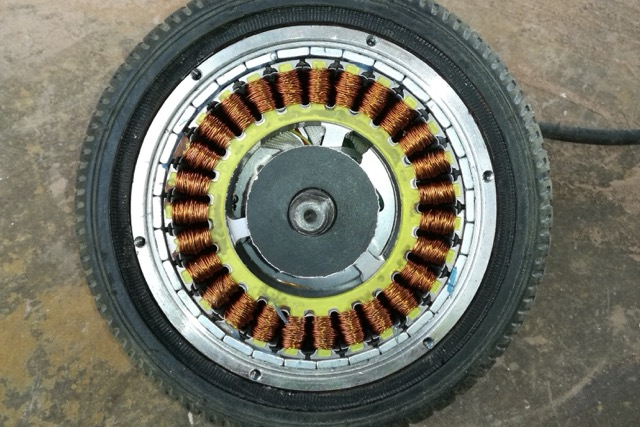
\includegraphics[width=0.5\textwidth]{fig/lec01/Wheel_hub_PMSM.jpg}
			\caption{Permanent magnet machine (source: \href{https://commons.wikimedia.org/wiki/File:Wheel_hub_motor_of_an_electric_kick_scooter,_sidepanel_removed_(2022).jpg}{Wikimedia Commons}, Andrez, \href{https://creativecommons.org/licenses/by-sa/4.0/deed.en}{CC BY-SA 4.0})}
		\end{subfigure}
		\hfill
		\begin{subfigure}[b]{0.49\textwidth}
			\centering
			\includegraphics[width=0.5\textwidth]{fig/lec01/Linear_motor.jpg}
			\caption{Linear permanent magnet machine (source: \href{https://commons.wikimedia.org/wiki/File:Linear_motor_by_Zureks.jpg}{Wikimedia Commons}, Zureks, \href{https://creativecommons.org/licenses/by-sa/4.0/n}{CC BY-SA 4.0})}
		\end{subfigure}
		\caption*{Some exemplary electrical machines} 
        \label{fig:examples_machine_drives_00}
	\end{figure}
\end{frame}


%%%%%%%%%%%%%%%%%%%%%%%%%%%%%%%%%%%%%%%%%%%%%%%%%%%%%%%%%%%%%
%% The machine as an electrical-mechanical converter %%
%%%%%%%%%%%%%%%%%%%%%%%%%%%%%%%%%%%%%%%%%%%%%%%%%%%%%%%%%%%%%
\begin{frame}
	\frametitle{The machine as an electrical-mechanical converter}
	\begin{figure}
		\centering
		\begin{subfigure}[b]{0.49\textwidth}
			\centering
			\includegraphics[width=0.9\textwidth]{fig/lec01/Block_diagram_rotational_converter.pdf}
			\caption{Rotational converter}
		\end{subfigure}
		\hfill
		\begin{subfigure}[b]{0.49\textwidth}
			\centering
			\includegraphics[width=0.9\textwidth]{fig/lec01/Block_diagram_translational_converter.pdf}
			\caption{Translational converter}
		\end{subfigure}
		\caption{Electrically and mechanically free body diagrams of motors as energy converters  with variable notation: time $t$, voltage $u$, current $i$, force $F$, displacement $x$, torque $T$ and rational speed $\omega$ (adapted from J.~B\"ocker, \textit{Elektrische Antriebstechnik}, Paderborn University, 2020)} 
        \label{fig:free_body_diagrams_motor}
	\end{figure}
\end{frame}

%%%%%%%%%%%%%%%%%%%%%%%%%%%%%%%%%%%%%%%%%%%%%%%%%%%%%%%%%%%%%
%% Some basic mechanical terms (recap) %%
%%%%%%%%%%%%%%%%%%%%%%%%%%%%%%%%%%%%%%%%%%%%%%%%%%%%%%%%%%%%%
\begin{frame}
	\frametitle{Some basic mechanical terms (recap)}
	\vspace{-0.15cm}
	\begin{table}
		\centering
		\begin{tabular}{lll}
			& Translational converter & Rotational converter \\
			\toprule
			Kinematic quantities & & \\
			Displacement / angle & $x$ & $\varepsilon$ \\
			Velocity & $v=\dot{x}$ & $\omega=\dot{\varepsilon}$ \\
			Acceleration & $a=\dot{v}=\ddot{x}$ & $\alpha=\dot{\omega}=\ddot{\varepsilon}$ \\
			Jerk & $j=\dot{a}=\ddot{v}=\dddot{x}$ & $\rho=\dot{\alpha}=\ddot{\omega}=\dddot{\varepsilon}$ \onslide<2-> \\
			\midrule
			Dynamical quantities & & \\
			Force / torque & $F$ & $T$ \\
			Mass / inertia & $m$ & $J$ \onslide<3-> \\
			\midrule
			Mechanical power & $P_\mathrm{me}=F v$ & $P_\mathrm{me}=T \omega$ \onslide<4-> \\
			Work & $W[t_0,t]=\int_{t_0}^t P_\mathrm{me}(\tau)\,\mathrm{d}\tau$ & $W[t_0,t]=\int_{t_0}^t P_\mathrm{me}(\tau)\,\mathrm{d}\tau$ \onslide<5-> \\
			Momentum / rotational momentum & $p = m v$ & $L = \omega J$ \onslide<6-> \\
			Kinetic energy & $E_\mathrm{kin} = \frac{1}{2} m v^2$ & $E_\mathrm{kin} = \frac{1}{2} J \omega^2$\\
			\bottomrule
		\end{tabular}
		\caption{Basic mechanical terms for translational and rotational converters}
		\label{tab:basic_mechanical_terms}
	\end{table}
\end{frame}

%%%%%%%%%%%%%%%%%%%%%%%%%%%%%%%%%%%%%%%%%%%%%%%%%%%%%%%%%%%%%
%% Work vs. energy (recap) %%
%%%%%%%%%%%%%%%%%%%%%%%%%%%%%%%%%%%%%%%%%%%%%%%%%%%%%%%%%%%%%
\begin{frame}
	\frametitle{Work vs. energy (recap)}
	\begin{columns}
		\begin{column}{0.5\textwidth}
			\begin{varblock}{Work}
				Work is the integral of the power over a time integral (or force over distance) and is a measure of the energy transfer.
			\end{varblock}
		\end{column}
		\begin{column}{0.5\textwidth}
			\begin{varblock}{Energy}
				Energy is the capacity to do work, that is, a quantity depending on the state of a system at a given point of time.				
			\end{varblock}
		\end{column}
		\end{columns}
		\vspace{0.5cm}
		\begin{figure}
			\centering
			\includegraphics[width=0.6\textwidth]{fig/lec01/Work_Energy.pdf}
			\caption{Illustration addressing the work vs. energy terminology (simplified Sankey diagram)}
			\label{fig:work_vs_energy}
		\end{figure}
\end{frame}

%%%%%%%%%%%%%%%%%%%%%%%%%%%%%%%%%%%%%%%%%%%%%%%%%%%%%%%%%%%%%
%% Power balance of an electrical machine %%
%%%%%%%%%%%%%%%%%%%%%%%%%%%%%%%%%%%%%%%%%%%%%%%%%%%%%%%%%%%%%
\begin{frame}
	\frametitle{Power balance of an electrical machine}
	\begin{figure}
		\centering
		\includegraphics[width=0.45\textwidth]{fig/lec01/Power_balance_machine.pdf}
		\caption{Power balance of an electrical machine (illustrated in motoric operation)}
		\label{fig:power_balance_machine}
	\end{figure}
	The power balance
	\begin{equation}
		P_\mathrm{el}(t) = P_\mathrm{me}(t) + P_\mathrm{l}(t) + \frac{\mathrm{d}}{\mathrm{d}t}E_\mathrm{i}(t)
	\end{equation}
	must hold for any point in time as energy is conserved, that is, not created or destroyed.
\end{frame}

%%%%%%%%%%%%%%%%%%%%%%%%%%%%%%%%%%%%%%%%%%%%%%%%%%%%%%%%%%%%%
%% Four quadrants of machine operation %%
%%%%%%%%%%%%%%%%%%%%%%%%%%%%%%%%%%%%%%%%%%%%%%%%%%%%%%%%%%%%%
\begin{frame}
	\frametitle{Four quadrants of machine operation}
	\begin{columns}
		\begin{column}{0.5\textwidth}
			For the steady state ($\dot{E}_{\mathrm{i}}(t)=0$), we define the \hl{machine efficiency} as the ratio of the converted energy to the input energy:
			\begin{align}
				\eta_\mathrm{mot} &= \frac{P_{\mathrm{me}}}{P_{\mathrm{el}}} = 1- \frac{P_{\mathrm{l}}}{P_{\mathrm{el}}},  \\[0.5em] 
				\onslide<2->{\eta_\mathrm{gen} &= \frac{P_{\mathrm{el}}}{P_{\mathrm{me}}} = 1- \frac{P_{\mathrm{l}}}{P_{\mathrm{me}}}.}
			\end{align}
			\onslide<3->{Hence, we need to consider in which \hl{quadrant} the machine operates as this will influence the power flow direction.}
		\end{column}
		\begin{column}{0.5\textwidth}
			\onslide<3->\begin{figure}
				\centering
				\includegraphics[width=0.75\textwidth]{fig/lec01/Machine_quadrants.pdf}
				\caption{Machine quadrants (derived from \href{https://de.wikipedia.org/wiki/Datei:Vierquadranten.svg}{Wikimedia Commons}, K. Pitter, \href{https://creativecommons.org/licenses/by-sa/3.0/deed.de}{CC BY-SA 3.0})}
				\label{fig:machine_quadrants}
			\end{figure}
		\end{column}
		\end{columns}
\end{frame}


%%%%%%%%%%%%%%%%%%%%%%%%%%%%%%%%%%%%%%%%%%%%%%%%%%%%%%%%%%%%%
%% What is an electrical drive ? %%
%%%%%%%%%%%%%%%%%%%%%%%%%%%%%%%%%%%%%%%%%%%%%%%%%%%%%%%%%%%%%
\begin{frame}
	\frametitle{What is an electrical drive ?}
	\begin{columns}
		\begin{column}{0.4\textwidth}
			\begin{varblock}{Electrical drive}
			   An electrical drive is a system that controls the torque, speed or position of an electrical machine connected to some mechanical process.
			\end{varblock}
			\vspace{0.25cm}
			\begin{itemize}
				\item<2-> Integrates the 'stupid' electrical machine into an 'intelligent' controlled system.
				\item<3-> The energy source and mechanical process ('load') are not part of the drive system.
			\end{itemize}
		\end{column}
		\begin{column}{0.6\textwidth}
			\begin{figure}
				\centering
				\includegraphics[width=0.95\textwidth]{fig/lec01/Electrical_Drive_Block_Overview.pdf}
				\caption{Block diagram of an electrical drive (adapted from J.~B\"ocker, \textit{Elektrische Antriebstechnik}, Paderborn University, 2020)}
			\end{figure}
		\end{column}
	\end{columns}
\end{frame}

%%%%%%%%%%%%%%%%%%%%%%%%%%%%%%%%%%%%%%%%%%%%%%%%%%%%%%%%%%%%%
%% Examples of electrical machine and drive applications (1) %%
%%%%%%%%%%%%%%%%%%%%%%%%%%%%%%%%%%%%%%%%%%%%%%%%%%%%%%%%%%%%%
\begin{frame}
	\frametitle{Examples of electrical machine and drive applications (1)}
	\begin{figure}
		\centering
		\begin{subfigure}[b]{0.49\textwidth}
			\centering
			\includegraphics[width=0.5\textwidth]{fig/lec01/Electric_Car_recharging.jpg}
			\caption{Electric cars (source: \href{https://commons.wikimedia.org/wiki/File:Electric_Car_recharging.jpg}{Wikimedia Commons}, M.~Movchin and F. Mueller, \href{https://creativecommons.org/licenses/by-sa/3.0/deed.en}{CC BY-SA 3.0})}
		\end{subfigure}
		\hfill
		\begin{subfigure}[b]{0.49\textwidth}
			\centering
			\includegraphics[width=0.5\textwidth]{fig/lec01/sky-farm-windmill.jpg}
			\caption{Wind turbine generators (source: \href{https://pxhere.com/en/photo/954757}{pxhere.com}, public domain)}
		\end{subfigure}
		\\
		\begin{subfigure}[b]{0.49\textwidth}
			\centering
			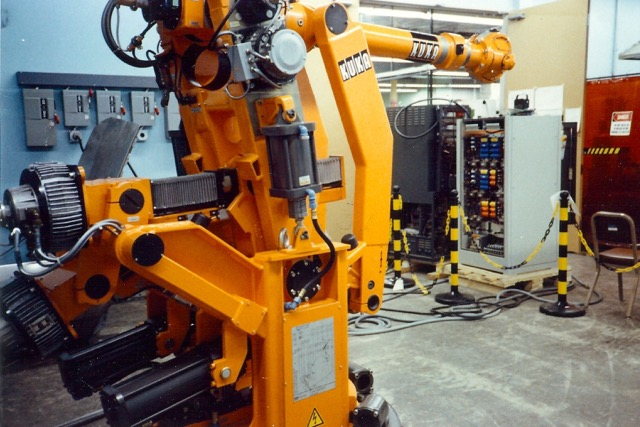
\includegraphics[width=0.5\textwidth]{fig/lec01/Automatix_KukaRobot.jpg}
			\caption{Factory robots (source: \href{https://commons.wikimedia.org/wiki/File:Automatix_KukaRobot483.agr.jpg}{Wikimedia Commons}, A.~Reinhold, \href{https://creativecommons.org/licenses/by-sa/4.0/deed.en}{CC BY-SA 4.0})}
		\end{subfigure}
		\hfill
		\begin{subfigure}[b]{0.49\textwidth}
			\centering
			\includegraphics[width=0.5\textwidth]{fig/lec01/electric_drill.jpg}
			\caption{Electric tools (source: \href{https://www.flickr.com/photos/30478819@N08/49940384798}{flickr.com},  M.~Verch, \href{https://creativecommons.org/licenses/by/2.0/}{CC BY 2.0})}
		\end{subfigure}
		\caption*{Examples of electrical machine and drive applications} 
        \label{fig:examples_machine_drives_01}
	\end{figure}
\end{frame}

%%%%%%%%%%%%%%%%%%%%%%%%%%%%%%%%%%%%%%%%%%%%%%%%%%%%%%%%%%%%%
%% Examples of electrical machine and drive applications (2) %%
%%%%%%%%%%%%%%%%%%%%%%%%%%%%%%%%%%%%%%%%%%%%%%%%%%%%%%%%%%%%%
\begin{frame}
	\frametitle{Examples of electrical machine and drive applications (2)}
	% Set up a 2x2 grid of figures
	\begin{figure}
		\ContinuedFloat
		\centering
		\begin{subfigure}[b]{0.49\textwidth}
			\centering
			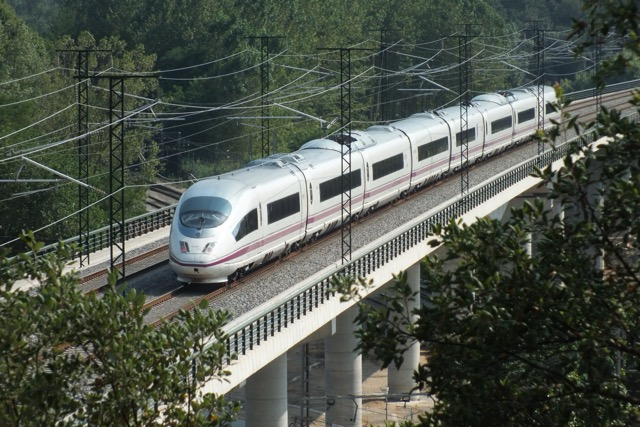
\includegraphics[width=0.5\textwidth]{fig/lec01/Train.jpg}
			\caption{High-speed trains (source: \href{https://commons.wikimedia.org/wiki/File:Fast_Train_Spain_Class_103_AVE_Siemens_Bridge_Macanet-Massanes.JPG}{Wikimedia Commons}, P.~Elektro, \href{https://creativecommons.org/licenses/by-sa/3.0/deed.en}{CC BY-SA 3.0})}
		\end{subfigure}
		\hfill
		\begin{subfigure}[b]{0.49\textwidth}
			\centering
			\includegraphics[width=0.5\textwidth]{fig/lec01/Electric_Airbus_A320.jpg}
			\caption{Electric aircrafts (source: \href{https://commons.wikimedia.org/wiki/File:Electric_Airbus_A320.jpg}{Wikimedia Commons}, M.~Weinold, \href{https://creativecommons.org/licenses/by-sa/4.0/deed.en}{CC BY-SA 4.0})}
		\end{subfigure}
		\\
		\begin{subfigure}[b]{0.49\textwidth}
			\centering
			\includegraphics[width=0.5\textwidth]{fig/lec01/Pump.jpg}
			\caption{Pumps (source: \href{https://commons.wikimedia.org/wiki/File:Hammelmann_Stationary_unit_with_electric_motor.jpg}{Wikimedia Commons}, Hammelmann, \href{https://creativecommons.org/licenses/by-sa/3.0/deed.en}{CC BY-SA 3.0})}
		\end{subfigure}
		\hfill
		\begin{subfigure}[b]{0.49\textwidth}
			\centering
			\includegraphics[width=0.5\textwidth]{fig/lec01/crane.jpg}
			\caption{Cranes (source: \href{https://commons.wikimedia.org/wiki/File:Hammelmann_Stationary_unit_with_electric_motor.jpg}{Wikimedia Commons}, Belfast Dissenter, \href{https://creativecommons.org/licenses/by-sa/4.0/deed.en}{CC BY-SA 4.0})}
		\end{subfigure}
		\caption*{Examples of electrical machine and drive applications} 
        \label{fig:examples_machine_drives_02}
	\end{figure}
\end{frame}

%%%%%%%%%%%%%%%%%%%%%%%%%%%%%%%%%%%%%%%%%%%%%%%%%%%%%%%%%%%%%
%% Examples of electrical machine and drive applications (2) %%
%%%%%%%%%%%%%%%%%%%%%%%%%%%%%%%%%%%%%%%%%%%%%%%%%%%%%%%%%%%%%
\begin{frame}
	\frametitle{A broad range of nominal power ratings}
	\vspace{-0.1cm}
	\begin{figure}
		\centering
		\includegraphics[height=0.7\textheight]{fig/lec01/Power_Classes_Examples.pdf}
		\caption{Power range overview (inspired  from A.~Binder, \textit{Elektrische Maschinen und Antriebe (lecture slides)}, Darmstadt University, 2022 with additional figure sources: \href{https://www.flickr.com/photos/arthurwolf/5393520058/}{A. Wolf}, \href{https://commons.wikimedia.org/wiki/File:Wald_am_Arlberg-OeBB_Spullersee_power_plant-M1-Rotor-11ASD.jpg}{Asurnipal}, \href{https://www.flickr.com/photos/mouser-nerdbot/7042785635}{M. Williams}, \href{https://de.m.wikipedia.org/wiki/Datei:Stick_blender_Electrolux_AEG_HB_9807_-_stator_of_the_electric_motor-4313.jpg}{R. Spekking}, \href{https://commons.wikimedia.org/wiki/File:Electric_motor_and_transmission_in_a_truck.jpg}{Foxcorner}, \href{https://commons.wikimedia.org/wiki/File:E-bike_electric_motor_shimano_ep_8.jpg}{A.~Tredz} and \href{https://commons.wikimedia.org/wiki/File:2023_Corsair_SP120_RGB_Elite.jpg}{J. Halicki} under varying CC licenses) }
		\label{Power_Classes_Examples}
	\end{figure}
\end{frame}

%%%%%%%%%%%%%%%%%%%%%%%%%%%%%%%%%%%%%%%%%%%%%%%%%%%%%%%%%%%%%
%% Why are electric machines and drives important ? %%
%%%%%%%%%%%%%%%%%%%%%%%%%%%%%%%%%%%%%%%%%%%%%%%%%%%%%%%%%%%%%
\begin{frame}
	\frametitle{Why is knowledge about electric machines and drives important?}
	\begin{varblock}{Electric machines and drives are an essential pillar of the modern society}
		Without electric machines and drives, our todays' society would not be possible. Starting from providing electricity via electrical generators to powering electric vehicles, tools and entire factory production lines, electric machines and drives are everywhere, that is, they enable our today's living standard. 
	\end{varblock}
	\begin{varblock}{Energy efficiency and sustainability is key}<2->
		Electric machines and drives utilize  approx. 50\,\% of the global electricity with about 8 billion electric motors in use in the EU (source: \href{https://commission.europa.eu/energy-climate-change-environment/standards-tools-and-labels/products-labelling-rules-and-requirements/energy-label-and-ecodesign/energy-efficient-products/electric-motors-and-variable-speed-drives_en}{European Commission} and \href{https://iea.blob.core.windows.net/assets/d69b2a76-feb9-4a74-a921-2490a8fefcdf/EE_for_ElectricSystems.pdf}{International Energy Agency}). Therefore, improving their efficiency is an essential factor to reduce the global energy consumption and the associated CO$_2$ emissions.
	\end{varblock}
\end{frame}

%%%%%%%%%%%%%%%%%%%%%%%%%%%%%%%%%%%%%%%%%%%%%%%%%%%%%%%%%%%%%
%% Learning objectives %%
%%%%%%%%%%%%%%%%%%%%%%%%%%%%%%%%%%%%%%%%%%%%%%%%%%%%%%%%%%%%%
\begin{frame}
	\frametitle{Learning objectives}
	\begin{itemize}
		\item Understand the generation of magnetic fields, force formation and voltage induction in electrical machines.
		\item<2-> Differentiate the main types of electrical machines and drives:
		\begin{itemize}
			\item DC machines. 
			\item Induction machines.
			\item Synchronous machines.
			\item And their plentiful variants \ldots
		\end{itemize}
		\item<3-> Understand their basic design and operation principles.
		\item<4-> Analyze the operation of electrical machines and drives:
		\begin{itemize}
			\item in steady state and
			\item in transient conditions.
		\end{itemize} 
		\item<5-> Have fun learning about electrical machines and drives.
	\end{itemize}
\end{frame}

%%%%%%%%%%%%%%%%%%%%%%%%%%%%%%%%%%%%%%%%%%%%%%%%%%%%%%%%%%%%%
%% Necessary prior knowledge %%
%%%%%%%%%%%%%%%%%%%%%%%%%%%%%%%%%%%%%%%%%%%%%%%%%%%%%%%%%%%%%
\begin{frame}
	\frametitle{Necessary prior knowledge for this course}
	You should have a basic understanding of the following topics:
	\begin{itemize}
		\item Linear differential equations (modeling, solution techniques)
		\item Linear algebra basics (e.g., vector and matrix operations)
		\item Vector analysis (differentiation and integration of vector fields)
		\item Basic signal theory knowledge (e.g., Fourier series, Laplace transform)
		\item Basic knowledge of electrical circuit theory
		\item Basic knowledge of mechanics
	\end{itemize}
	\vspace{0.5cm}
	\onslide<2->What we will \underline{not} cover, that is, you do not need to know (covered in separate courses):
	\begin{itemize}
		\item Control engineering (design drive controllers)
		\item Power electronics (design switchable actuators)
	\end{itemize}
\end{frame}

%%%%%%%%%%%%%%%%%%%%%%%%%%%%%%%%%%%%%%%%%%%%%%%%%%%%%%%%%%%%%
%% Recommended reading %%
%%%%%%%%%%%%%%%%%%%%%%%%%%%%%%%%%%%%%%%%%%%%%%%%%%%%%%%%%%%%%
\begin{frame}
	\frametitle{Recommended reading}
	\begin{itemize}
		\item A. Binder, Elektrische Maschinen und Antriebe (in German), Vol. 2, Springer, 2017
		\item D. Schr\"oder and R. Kennel, Elektrische Antriebe: Grundlagen (in German), Vol. 7, Springer Vieweg, 2021
		\item A. Huges and B. Drury, Electric Motors and Drives: Fundamentals, Types and Applications, Vol. 5, Newnes, 2019
		\item S. Chapman, Electric Machinery Fundamentals, Vol. 5, McGraw-Hill, 2011
		\item I. Boldea and S. Nasar, Electric Drives, Vol. 3, CRC Press, 2022
	\end{itemize}
\end{frame}